\documentclass[a4paper,12pt]{article}

\usepackage[margin=1in]{geometry} % full-width

% AMS Packages
\usepackage{amsmath}
\usepackage{amsthm}
\usepackage{amssymb}

% Unicode
\usepackage[utf8]{inputenc}
\usepackage{hyperref}
\hypersetup{
    unicode,
    colorlinks,
%   breaklinks,
%   urlcolor=cyan,
    linkcolor=blue,
    pdfauthor={Author One, Author Two, Author Three},
    pdftitle={A simple article template},
    pdfsubject={A simple article template},
    pdfkeywords={article, template, simple},
    pdfproducer={LaTeX},
    pdfcreator={pdflatex}
}

% Vietnamese
%\usepackage{vntex}

% Natbib
\usepackage[sort&compress,numbers,square]{natbib}
\bibliographystyle{plain}

% Theorem, Lemma, etc
% \theoremstyle{plain}
% \newtheorem{theorem}{Theorem}
% \newtheorem{corollary}[theorem]{Corollary}
% \newtheorem{lemma}[theorem]{Lemma}
% \newtheorem{claim}{Claim}[theorem]
% \newtheorem{axiom}[theorem]{Axiom}
% \newtheorem{conjecture}[theorem]{Conjecture}
% \newtheorem{fact}[theorem]{Fact}
% \newtheorem{hypothesis}[theorem]{Hypothesis}
% \newtheorem{assumption}[theorem]{Assumption}
% \newtheorem{proposition}[theorem]{Proposition}
% \newtheorem{criterion}[theorem]{Criterion}
% \theoremstyle{definition}
% \newtheorem{definition}[theorem]{Definition}
% \newtheorem{example}[theorem]{Example}
% \newtheorem{remark}[theorem]{Remark}
% \newtheorem{problem}[theorem]{Problem}
% \newtheorem{principle}[theorem]{Principle}

\usepackage{graphicx, color}
\graphicspath{{figures/}}

%\usepackage[linesnumbered,ruled,vlined,commentsnumbered]{algorithm2e} % use algorithm2e for typesetting algorithms
\usepackage{algorithm, algpseudocode} % use algorithm and algorithmicx for typesetting algorithms
\usepackage{mathrsfs} % for \mathscr command

\usepackage{lipsum}

% Author info
\title{Exposé on Using Large Language Models for Automated Data Extraction from Scientific Literature}
\author{Felix Karg}

\date{\today}
% \renewcommand{\abstractname}{\vspace{-\baselineskip}} % clear 'abstract' from abstract

\newcommand{\margtodo}                                 % used by \todo command
{\marginpar{\textbf{\textcolor{red}{ToDo}}}{}}
\newcommand{\todo}[1]
{{\textbf{\textcolor{red}{[\margtodo{}#1]}}}{}}   % for todo-notes inside 


\begin{document}
\maketitle

% \begin{abstract}

    % \noindent\textbf{Keywords:} article, template, simple
% \end{abstract}

% \tableofcontents

\section{Introduction}
A large amount of scientific knowledge is scattered across millions of research
papers. Often, this research is not in standardized machine-readable formats,
which makes it difficult or impossible to build on prior work using powerful
tools to extract further knowledge.  % \todo{expand on LLMs and limits here?}
% setting up and running llm individually is expensive in time and compute

\section{Motivation}
Take for example the field of synthesizing Metal-Organic Frameworks (MOFs)
\cite{zhou_introduction_2012}. While numerous detailed descriptions of
synthesis procedures exist, they are not in a machine-readable format, which
prevents effective application of state-of-the-art techniques such as automated
experimentation \cite{shi_automated_2021} or synthesis prediction
\cite{luo_mof_2022}. Thus, we intend to create a pipeline for deriving
machine-readable information on MOF synthesis parameters from given questions
on provided scientific articles.


\section{Background}
\paragraph{Rule-Based Entity Recognition}
There have long been rule-based approaches for the recognition of individual
entities. ChemTagger \cite{hawizy_chemicaltagger_2011} clearly demonstrated
that simple rule-based systems can sometimes extract much of the requested
information. While they often achieve high precision for simple tasks,
they fail in answering more complex queries, such as the relation between
two entities.

\paragraph{Language Models}
With 'Attention is All you Need' \cite{vaswani_attention_2017}, Google
introduced the transformer architecture for language models and demonstrated
significant improvements. Soon, BERT \cite{devlin_bert_2018} followed, a model
which is conceptually simple and empirically powerful. It was soon demonstrated
that BERT can be easily fine-tuned for named entity recognition in materials
science \cite{zhao_finetuning_2021}. OpenAI pushed scaling forward with their
GPT2 \cite{radford_language_2019} model, which was substantially larger than
BERT. Step-by-step, these models enabled more sophisticated extraction requests.

\paragraph{Large Language Models}
With the introduction of GPT3 \cite{brown_language_2020} OpenAI trailblazed the
era of Large Language Models. This model enabled more sophisticated information
extraction requests with little fine-tuning \cite{dunn_structured_2022}. Soon,
open-source variants such as OPT \cite{zhang_opt_2022} followed. It was also
demonstrated with Chinchilla \cite{hoffmann_training_2022} and CoTR
\cite{zhang_multimodal_2023}, that these large language models are
substantially overparametrized and undertrained.

% \paragraph{Downstream Usages}
% MOF Synthesis Prediction Enabled by Automatic Data Mining and Machine Learning \cite{luo_mof_2022}
% Doing Synthesis prediction based on an automatic data extraction pipeline
% \todo{rewrite}

\section{Scientific Questions}
Use Large Language Models to demonstrate automated extraction of unstructured
text from scientific literature for the creation of a database with otherwise
unavailable information on MOF synthesis. By doing so, we create a pipeline
that can easily be adapted to numerous other data extraction tasks.

Specifically, using OPT \cite{zhang_opt_2022} empirically test if accuracy can
be improved via 1) fine-tuning and 2) prompt engineering. Additionally,
test if 3) model size can be reduced by using distillation
\cite{sun_patient_2019}, and how it will affect accuracy as well as compute and
memory requirements. Distillation would enable considerable model parameter
reduction with little loss in accuracy, which could make it substantially
less compute intensive to fine-tune and run.

% Benchmarking accuracy of data extraction from scientific literature using state-of-the-art LLMs and other tools: how well do various existing methods do, and (how much) can priming, fine-tuning and prompt engineering improve this. \todo{rewrite}
% 
% Specifically, compare the accuracy of:
% \begin{itemize}
%     \item what the model already knows: here, the article would not be in context
%     \item what it can easily extract from the article: when provided in
%         context, how well it can answer questions relating the content.
%     \item particarly, without much prompt engineering or fine-tuning the model
%     \item with prompt engineering: attempt to increase accuracy by finding good prompts for that
%     \item after task-based fine-tuning (without context, in-context, and with or without good prompts)
%     \begin{itemize}
%         \item articles included in fine-tuning
%         \item articles not fine-tuned on
%         \item experiment with fine-tuning approaches
%     \end{itemize}
%     \item Models of varying sizes
%     \begin{itemize}
%         \item the varying sizes of available OPT-models \cite{zhang_opt_2022}
%         \item given enough time, try to use distillation \cite{sun_patient_2019} to compress the model parameter size
%     \end{itemize}
% \end{itemize}

% \section{Objectives}
% Objectives of the work (both mandatory objectives and optional additional objectives)

% \section{Intermediate Steps}
% Concrete work steps
% \begin{enumerate}
%     \item Take exemplary / arbitrary synthesis paper
%     \item get paragraph classification to work
%     \item figure out how to pass the relevant paragraphs as LLM context
%     \item determine accuracy of answering the given questions based on reference database
%     \item first without, later with prompt engineering and fine-tuning of the model
% \end{enumerate}
% \todo{combine with schedule}

\section{Schedule}
\begin{figure}[ht!]
    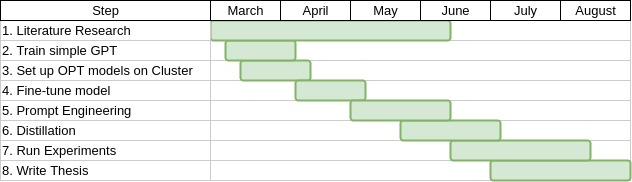
\includegraphics[width=\textwidth]{img/thesis_gantt}
    \caption{Exemplary timeline. Details are subject to change.}
\end{figure}

\subsection{Literature Research}
Get a better understanding by continuously reading relevant literature. This
includes articles mentioned here, but also others I may come across.

\subsection{Train Simple GPT}
Train a very small GPT model to get a deeper understanding of its architecture,
training procedure, and properties.

\subsection{Set up OPT models on Cluster}
While the OPT models are open source and can be downloaded, it might not be
trivial to set them up in the required configuration.

\subsection{Fine-tune model}
Construct and train the model on select examples, with intermediate annotations
or validation in-between, similiar to what is described in
\cite{dunn_structured_2022}. The goal is to increase task-success-rate
(answering in the requested machine-readable format) and accuracy.
\cite{dunn_structured_2022} have used 100 manual examples, and 500 partially
annotated ones to achieve high accuracy.

\subsection{Prompt Engineering}
Apply deep introspection and automatic prompt engineering \cite{zhou_large_2022}
in an attempt to increase the accuracy of generated databases.

\subsection{Distillation}
Apply distillation \cite{sun_patient_2019} to reduce model parameter size while
keeping accuracy high.

\subsection{Run Experiments}
Run detailed experiments and generate graphs, tables, and databases of extracted information.

\subsection{Write Thesis}
Write extensive scientific article as concluding work of my masters.

\bibliography{references.bib}
 
\end{document}
